\documentclass{article}

\usepackage[final]{neurips_2024}



\usepackage[utf8]{inputenc} % allow utf-8 input
\usepackage[T1]{fontenc}    % use 8-bit T1 fonts
\usepackage{hyperref}       % hyperlinks
\usepackage{url}            % simple URL typesetting
\usepackage{booktabs}       % professional-quality tables
\usepackage{amsfonts}       % blackboard math symbols
\usepackage{nicefrac}       % compact symbols for 1/2, etc.
\usepackage{microtype}      % microtypography
\usepackage{xcolor}         % colors
\usepackage{amsmath}
\usepackage{graphicx}
\usepackage{pythonhighlight}
\usepackage{subcaption}
\usepackage{float}

\newcommand{\todo}[1]{\textcolor{red}{#1}}

\newcommand{\R}{\mathbb{R}}
\newcommand\Tstrut{\rule{0pt}{2.6ex}}

\title{Efficient Attention}


\author{
  Sahil Chaudhary \\
  \And
  Mrigank Pawagi \\
  \And
  Rohit Jorige \\
  \And
  Jajapuram Nagasai \\
  % \And
  % Bachelor of Technology \\
  % Indian Institute of Science\\
  % \texttt{\{sahilc, mrigankp, rohitrj, nagasaij\}@iisc.ac.in}
}

\begin{document}


\maketitle


\begin{abstract}
   % \todo{(1) Introduce transformers. (2) Talk about time complexity and why linformer. (3) Introduce fine-tuning and need for LoRA. (4) Mention contributions (experiments)} \\ 

    The transformer architecture proposed by Vaswani et al. revolutionized sequence transduction with its novel ``Scaled Dot-Product Attention'' by outperforming previously dominant recurrent and convolutional models, while dispensing recurrence and convolutions entirely. However, these transformers are prohibitively slow for very long sequences due to their $\mathcal{O}(N^2)$ time complexity in the forward pass, where $N$ is the sequence length. Katharopoulos et al. expressed the self-attention in these transformers as a linear dot-product of kernel feature maps and made use of the associativity property of matrix products to reduce the complexity to $\mathcal{O}(N)$. In addition to these theoritical results, recent empirical results suggest that training of and inference from these models can be made faster and more scalable. One such technique, `Low-Rank Adaption' or LoRA has been proposed by Hu et al. based on previous theoretical results by Li et al. and Aghajanyan et al. LoRA has proven to be particularly valuable in scalable adaptation of pre-trained models to new tasks through fine-tuning. In this article, we will discuss the results mentioned above. Besides reproducing some of the experiments in these papers, our contributions include new experiments to explore these results. 
   
  % The Transformer Revolution: Efficiency, Scalability, and Adaptability in Natural Language Processing.
  %       This term paper explores the transformative impact of the Transformer architecture on Natural Language Processing (NLP). We begin by examining the original Transformer model from Vaswani et al. (2017), which revolutionized machine translation by solely relying on attention mechanisms, achieving superior performance and faster training compared to prior recurrent and convolutional models.
  %       Next, we delve into Shen et al. (2020)'s work on "Fast Autoregressive Transformers with Linear Attention." This paper addresses a key limitation of the original Transformer – its quadratic complexity for long sequences. By reformulating self-attention as a linear operation, the authors achieve dramatic speedups for autoregressive tasks while revealing an underlying connection between Transformers and recurrent neural networks.
  %       Finally, we explore  Madaan et al. (2023)'s "LoRA: Low Rank Adaptation of Large Language Models." This paper tackles the challenge of adapting massive pre-trained language models (like GPT-3) to specific tasks. LORA introduces a novel low-rank adaptation technique that significantly reduces the number of trainable parameters while maintaining or even improving performance compared to traditional fine-tuning.
  %       Overall, this paper investigates how the Transformer architecture has addressed key challenges in NLP, paving the way for more efficient, scalable, and adaptable models.
\end{abstract}



\section{Attention Architecture}
    Attention mechanisms have become an integral part of complex sequence modeling and transduction models in various task, allowing modeling of dependencies without regard to their distance in the input or output sequences.
    Let $x \in \R^{N \times F}$ denote a sequence of N feature vectors of dimensions 'F'. As proposed by Vaswani et. al., transformer is a function $T: \R^{N \times F} \rightarrow \R^{N \times F}$ defined by the composition of L transformer layers $T_1(\cdot),T_2(\cdot),\cdots,T_i(\cdot),\cdots,T_L(\cdot)$, where $T_i(\cdot)$
    is defined as:
    \begin{equation}
        T_i(x)=f_i(A_i(x)+x)
    \end{equation}
    The function $f_i(\cdot)$ transforms each feature independently and implemented with some layer of feedforward Network. $A_i(\cdot)$ is the heart of our transformer i.e. attention. 
    Query, Key and values are defined as follows:
    $Q=xW_Q$  where, $W_Q \in \R^{F \times D}$, then $Q \in \R^{N \times D}$, $K=xW_K$  where, $W_K \in \R^{F \times D}$, then $K \in \R^{N \times D}$, $V=xW_V$  where, $W_V \in \R^{F \times F}$, then $V \in \R^{N \times F}$.
    Let's measure the match using sim function, where $sim: \R^D \times \R^D \rightarrow \R_+$.
    According to definition of attention by vaswani,
    \begin{equation}
        A_i(x)=V'=\begin{bmatrix}
            \frac{\sum_{j=1}^{N}sim(Q_k,K_j)V_j}{\sum_{j=1}^{N}sim(Q_k,K_j)}
        \end{bmatrix}_{k \in \{N\}}
    \end{equation}
    Then the entries of this matrix is, $ \frac{\sum_{j=1}^{N}sim(Q_k,K_j)V_j}{\sum_{j=1}^{N}sim(Q_k,K_j)}.$. This is more generalized version of attention from whatever vaswani et. al came up with. If one just substitute the similarity function with $sim(q,k)=exp(\frac{q^TK}{\sqrt{D}})$, we get
    \begin{equation}
        A_i(x)=softmax(\frac{QK^T}{\sqrt{D}})V
    \end{equation}
    
\subsection{Transofrmers are RNNs}
The definition of attention in $eq^{n}-3$ is generic and can be use to define several other attention implementation. Now, its upto you to decide a function that mimics the properties of similarity function. This includes all kernels $K: \R^{D} \times \R^{D} \rightarrow \R_+$. So, entries of $A_i(x)$ would be $
            \frac{\sum_{j=1}^{N}K(Q_k,K_j)V_j}{\sum_{j=1}^{N}K(Q_k,K_j)}$
       
Given such a kernel with a feature representation $\Phi(x)$, we can rewrite 
each entries of $A_i(x)$ as,
\begin{equation}
    V'_k=\frac{\sum_{j=1}^{N}\Phi(Q_k)^T\Phi(K_j)V_j}{\sum_{j=1}^{N}\Phi(Q_k)^T\Phi(K_j)}=\frac{\Phi(Q_k)^T\sum_{j=1}^{N}\Phi(K_j)V_j^T}{\Phi(Q_k)^T\sum_{j=1}^{N}\Phi(K_j)}  
\end{equation}

Note that, the softmax attention has the computational cost of $O(N^2)$. On the other hand, the new kernel based attention only has computational cost of O(N).
Transformer architecture can be used to efficiently train autoregressive models by masking the attention computation. Let $S_k=\sum_{j=1}^{k}\Phi(K_j)V_j^T$ and $Z_k=\sum_{j=1}^{k}\Phi(K_j)$. i.e. 
\begin{equation}
    V'_k=\frac{\Phi(Q_k)^T\sum_{j=1}^{k}\Phi(K_j)V_j^T}{\Phi(Q_k)^T\sum_{j=1}^{k}\Phi(K_j)}=\frac{\Phi(Q_k)^TS_k}{\Phi(Q_k)^TZ_k}
\end{equation}

Note that, $S_k$ and $Z_k$ can be computed from $S_{k-1}$ and $Z_{k-1}$ in constant time. This motivates us to see relation between Linear Transformer and RNN. If Linear Transformer with the masking introduced is thought as RNN, we have two hidden states, viz. S and Z. Assume the value of S and Z to be 0 for recurrence. Then,
\begin{align*}
    &S_0=0,\text{ } S_k=S_{k-1}+\Phi(K_k)V_k^T=S_{k-1}+\Phi(x_kW_k)(x_kW_V)^T\\
    &Z_0=0,\text{ } Z_k=Z_{k-1}+\Phi(K_k)=Z_{k-1}+\Phi(x_kW_K)\\
    &T_i(x)=f_i(\begin{bmatrix}
        \frac{\Phi(x_kW_Q^T)S_k}{\Phi(x_kW_Q^T)Z_k}+x_k
    \end{bmatrix}_{k \in N})
\end{align*}
Theoretically, it just not only shows that linear transformer are better than softmax based transformer but also, it satisfies few of the properties of RNN which motivates us to experiment Transformer in autoregressive tasks.
\subsection{Experiments}
We experimented the linear transformer over image generation tasks. We evaluate the model on image generation with autoregressive transformers on the widely used MNIST dataset. The architecture for this experiment is same to Katharopoulos et. al. Thanks to Katharaopoulos et. al., we had pretrained model for MNIST. We test the model on random image generation and measured the time, image completion task and quality measurement and time difference. 
\begin{center}
    \begin{tabular}{c c c }
		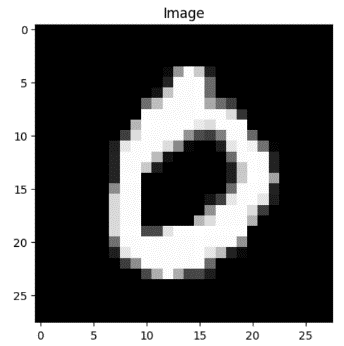
\includegraphics[width=0.15\textwidth]{images/input0.png} & 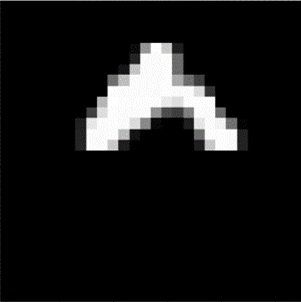
\includegraphics[width=0.15\textwidth]{images/occuluded0.png} & 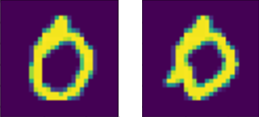
\includegraphics[width=0.3\textwidth]{images/result0.png} &  \\
		MNIST & Occuluded MNIST & Output
    \end{tabular}
\end{center}
    {Linear model was able to achieve faster and better image completion for given occluded input in comprasion to softmax based transformer}

\begin{tabular}{|c|c|c|c|}
    \hline
    S.No. & Number of Images generated & Linear & Softmax \\
    \hline
     1 & 100 & 33.45 & 367.91\\
     2 & 200 & 67.46 & 811.99\\
     3 & 300 & 76.46 & 1248.15\\
     4 & 400 & - & -\\
     5 & 500 & - & -\\
     \hline
\end{tabular}

To test the claim made for time complexity, we experimented on various length of random sequences for forward pass and backward pass in both of the models. We also experimented with the time taken to measure the attention in each of the case on random sequences only.
\begin{figure}
    \begin{subfigure}{0.5\textwidth}
        \centering
        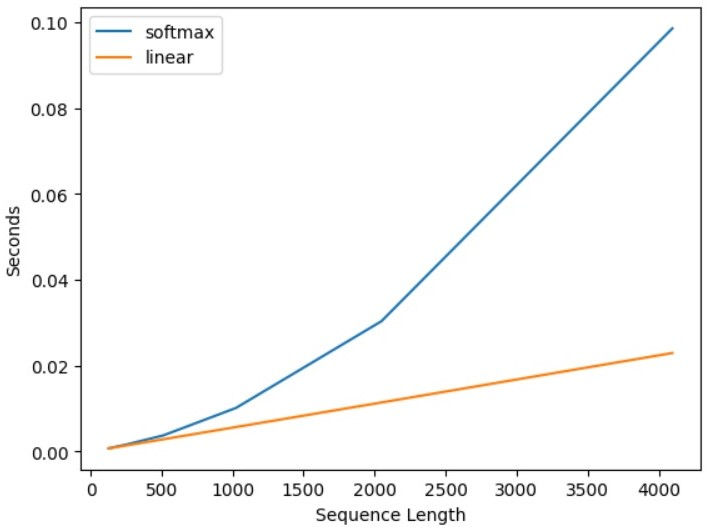
\includegraphics[scale=0.3]{images/forwardpassandbackwardpass.jpg}
        \caption{Time taken for forward pass and backward pass vs sequential length}
    \end{subfigure}
    \begin{subfigure}{0.5\textwidth}
        \centering
        
\includegraphics[scale=0.25]{images/bhosdiwala.jpg}
        \caption{Time taken for attention measure vs sequential length}
    \end{subfigure}
\end{figure}

\label{gen_inst}

\subsection{Occluded Image Completion}

\section{Low-Rank Adaptation (LoRA) of Large Language Models}
Due to the compute requirements of large-scale pre-training of Large Language Models (LLMs), fine-tuning is a widely adopted paradigm for adapting models pre-trained on general domain data to particular tasks or domains. However, the large number of parameters in such models can make even fine-tuning prohibitively expensive. Work from Li et al.~\cite{li2018measuring} and Aghajanyan et al.~\cite{aghajanyan2020intrinsic} has demonstrated that models may be over-parameterized and may reside on a low intrinsic dimension. Taking inspiration from these results, Hu et al.~\cite{hu2022lora} showed empirically that the change in weights during model adaptation also has a low intrinsic rank. This not only makes it possible to achieve comparable accuracies with faster fine-tuning (due to lesser trainable parameters) but also makes it possible to easily switch different adaptators in and out during deployment. A matrix $M \in \R^{n \times m}$ can be rank decomposed as $M = UV$ where $U \in \R^{n \times r}$, $V \in \R^{r \times m}$ and $r$ is the rank of $M$. This reduces the number of trainable parameters from $mn$ to $r(n + m)$. Note that $r(n + m) \ll nm$ for small $r$. This decomposition of the update matrices during fine-tuning lies at the heart of LoRA. Note that $r$ is not known \textit{a priori} and one may have to try several small values of $r$.

\subsection{Experiments}
We train a base neural network on an image classification task on the MNIST dataset. Our base model was composed of three linear layers which together had 55.1K trainable parameters. This model has a test accuracy of approximately 93.2\%. We then created our variants of MNIST, namely Quantized MNIST, Rotated MNIST, and Inverted MNIST. These are illustrated below through an example.

\begin{center}
    \begin{tabular}{c c c c}
		
\includegraphics[width=0.15\textwidth]{images/normal_5.png} & 
\includegraphics[width=0.15\textwidth]{images/quantized_5.png} & 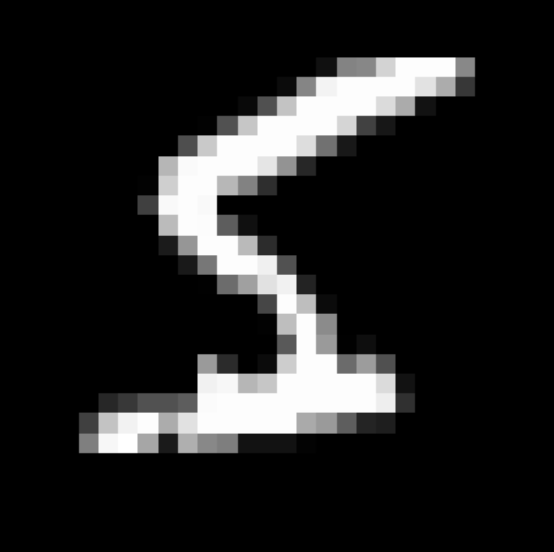
\includegraphics[width=0.15\textwidth]{images/rotated_5.png} & 
\includegraphics[width=0.15\textwidth]{images/inverted_5.png} \\
		MNIST & Quantized MNIST & Rotated MNIST & Inverted MNIST
    \end{tabular}
\end{center}

The accuracies of our base model on these modified datasets were approximately 85.58\%, 12.38\%, and 5.52\% respectively.


\subsubsection{Full Fine-Tuning}
We first fine-tuned our base model on the three datasets by modifying all 55.1K parameters. Our fine-tuned models achieved accuracies of approximately 93.57\%, 91.97\%, and 76.41\% on Quantized MNIST, Rotated MNIST, and Inverted MNIST respectively. These form our baselines for the fine-tuned models.

\subsubsection{Fine-Tuning with LoRA}
We then fine-tuned our base model on the three datasets using LoRA, with different values of $r$. We found that our fine-tuned models achieved accuracies comparable to their full fine-tuned counterparts with fewer trainable parameters. However due to the small size of our models, we could not observe any time improvements in training. The accuracies of our fine-tuned models in each domain and for each value of $r$ are given below.

\begin{center}
    \begin{tabular}{c | c | c | c | c}
        $r$ & Trainable Parameters & Quantized MNIST & Rotated MNIST & Inverted MNIST \\
        \hline
        % & & & & \\
        1 & 1.1K & 91.20\% & 37.53\% & 16.23\% \Tstrut \\
        2 & 2.1K & 91.30\% & 49.01\% & 17.92\% \\
        4 & 4.2K & 91.42\% & 69.10\% & 16.32\% \\
        8 & 8.4K & 91.39\% & 77.49\% & 32.19\% \\
        16 & 16.8K & 91.72\% & 86.95\% & 62.26\% \\
        32 & 33.6K & 92.31\% & 89.50\% & 68.06\% \\
        64 & 67.2K & 93.19\% & 90.41\% & 71.88\%
    \end{tabular}
\end{center}

\subsubsection{Full Training with LoRA}
We further explore whether LoRA can be used to train models from scratch, to observe if models have intrinsically low ranks. We trained separate models on each of our three modified MNIST datasets. The accuracies of these models are given below along with the respective $r$ values chosen.

\begin{center}
    \begin{tabular}{c | c | c | c | c}
        $r$ & Trainable Parameters & Quantized MNIST & Rotated MNIST & Inverted MNIST \\
        \hline
        % & & & & \\
        1 & 1.1K & 23.50\% & 25.91\% & 22.21\% \Tstrut \\
        2 & 2.1K & 37.48\% & 43.96\% & 45.81\% \\
        4 & 4.2K & 64.87\% & 62.60\% & 69.67\% \\
        8 & 8.4K & 77.96\% & 82.39\% & 83.11\% \\
        16 & 16.8K & 88.2\% & 86.76\% & 87.38\% \\
        32 & 33.6K & 90.13\% & 90.62\% & 90.25\% \\
        64 & 67.2K & 91.66\% & 91.85\% & 86.01\%
    \end{tabular}
\end{center}

\section{Acknowledgements}
We thank Dhruva Kashyap, one of the teaching assistants in UMC 203 and one of the last Emacs users, for his unwavering technical and emotional support throughout the preparation of this report.

\bibliographystyle{plain} % We choose the "plain" reference style
\bibliography{cite} % Entries are in the refs.bib file

\end{document}